\section{Behavior of Networks}

% \subsubsection{Controlled Experiments}

% \subsubsection{In the Wild}

% We ignore connections from the same network and ISP in which our servers were placed.


% \begin{figure}[t]
% 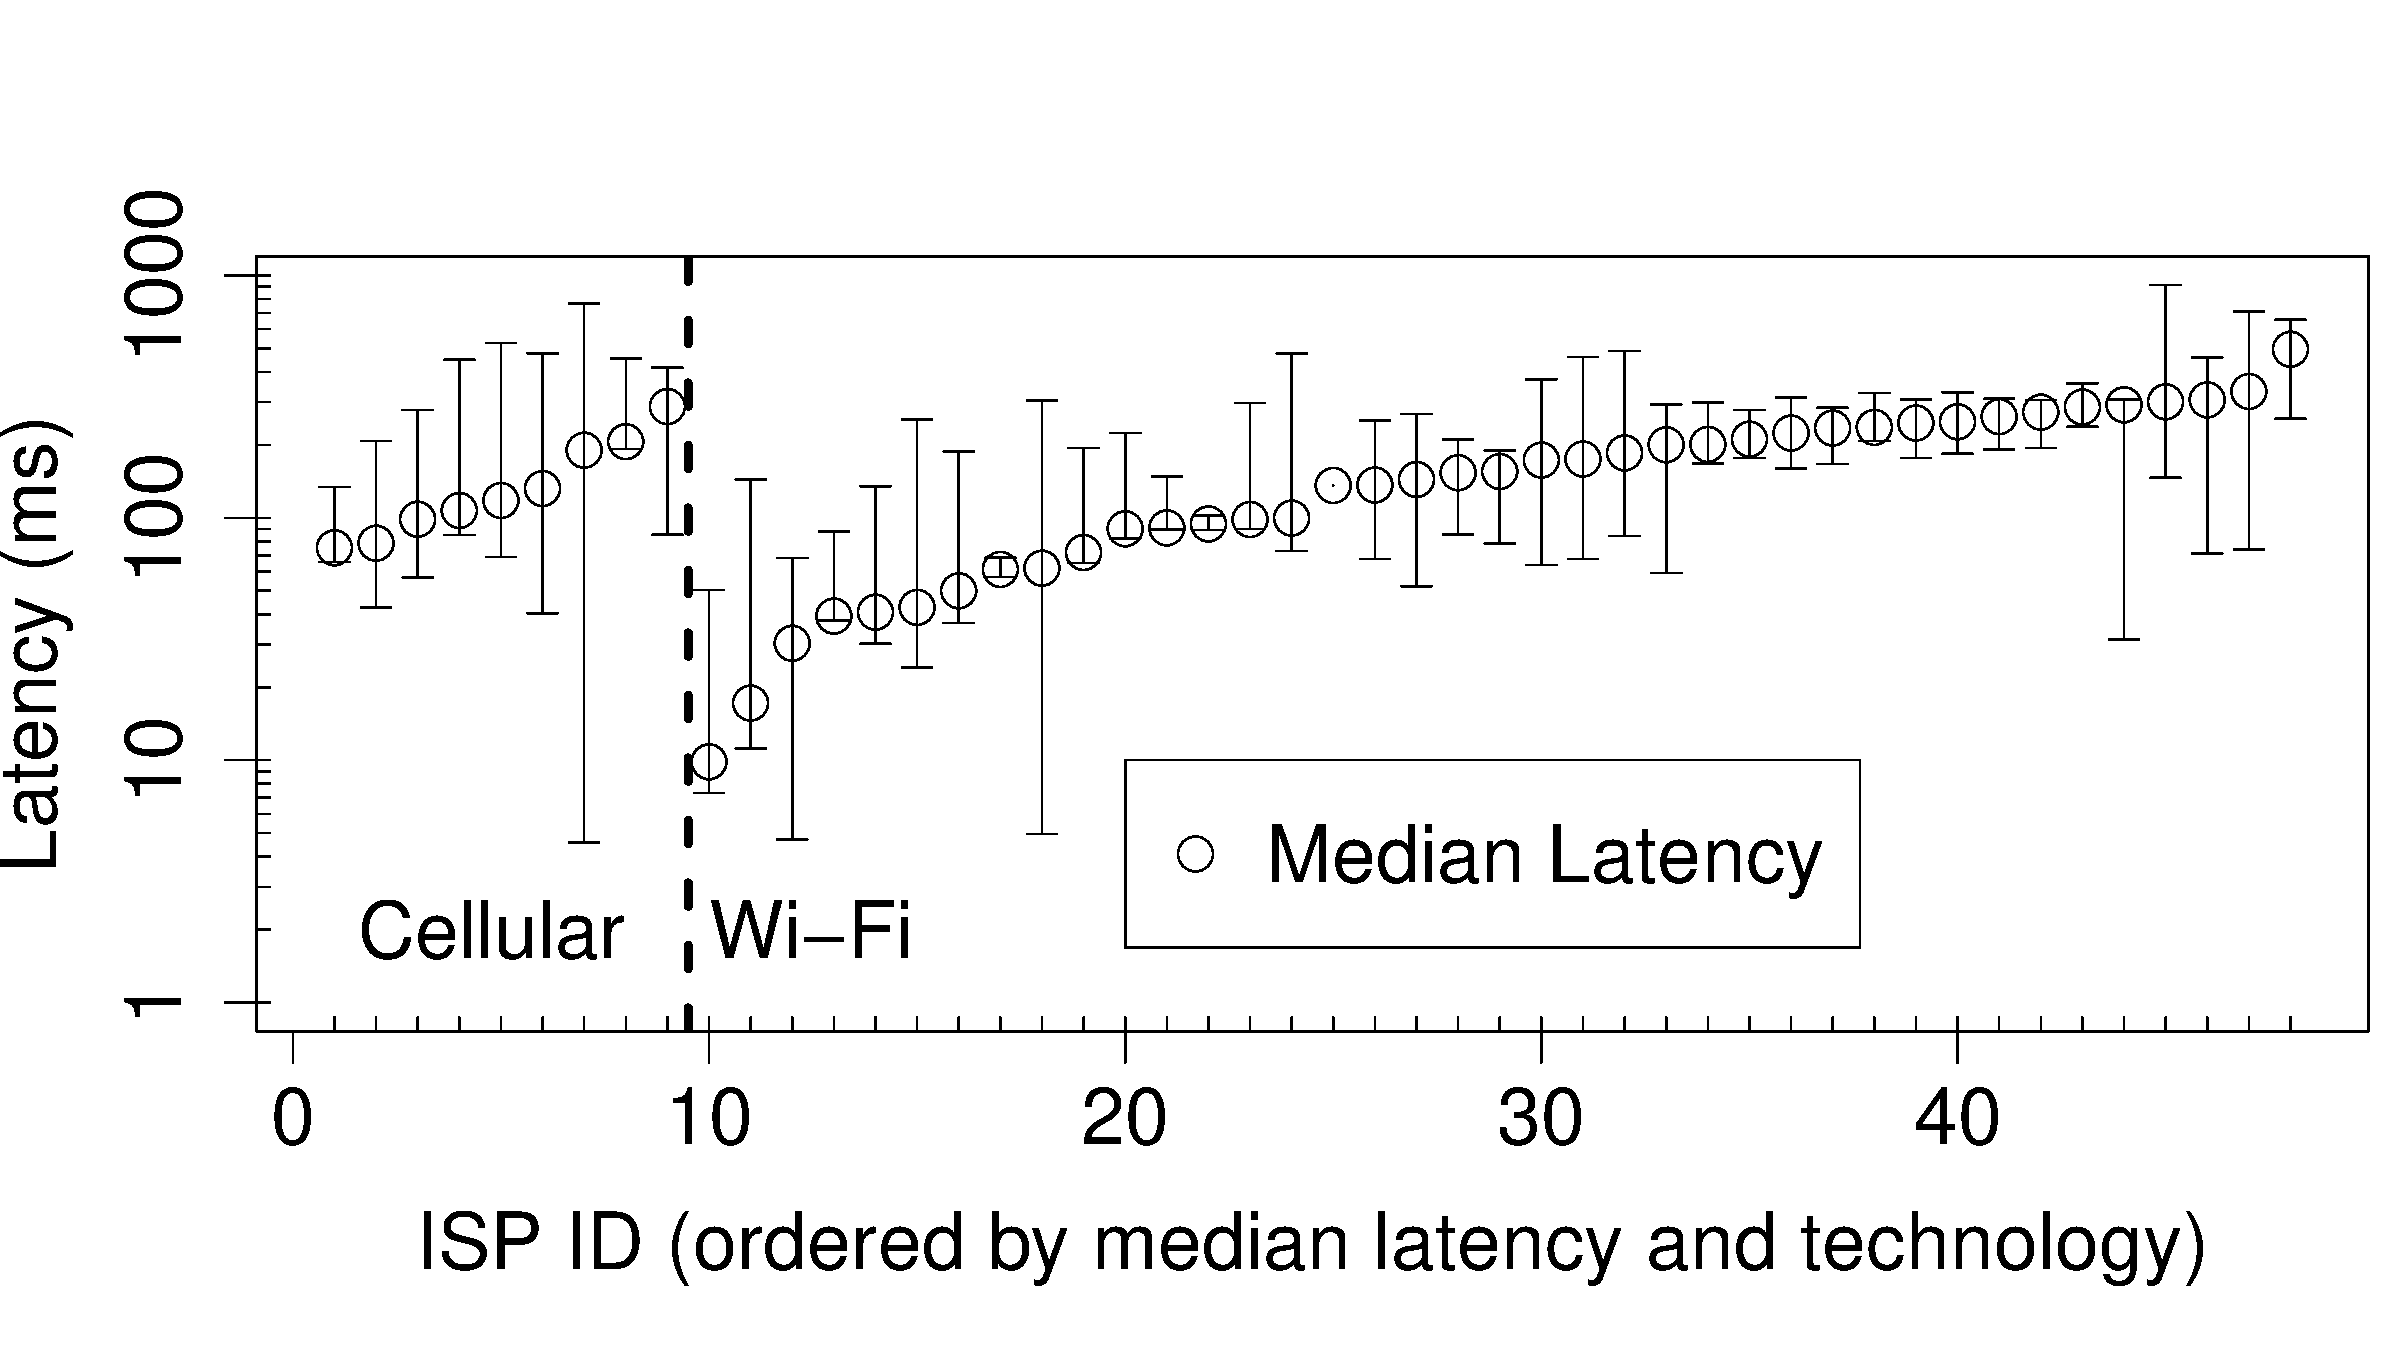
\includegraphics[width=\columnwidth]{plots/latency_isp_whisker.pdf}
% \caption{One-way latency from VPN server to mobile devices. \emph{Connections from cellular ISPs suffer a higher delay compared to Wi-Fi ISPs. The delays from Cellular ISPs is comparable to connecting from a Wi-Fi ISP in another country. Error bars indicate the 91st and 9th percentile}.}
% \label{fig:latency-across-isps}
% \end{figure}


% \begin{figure}[t]
% 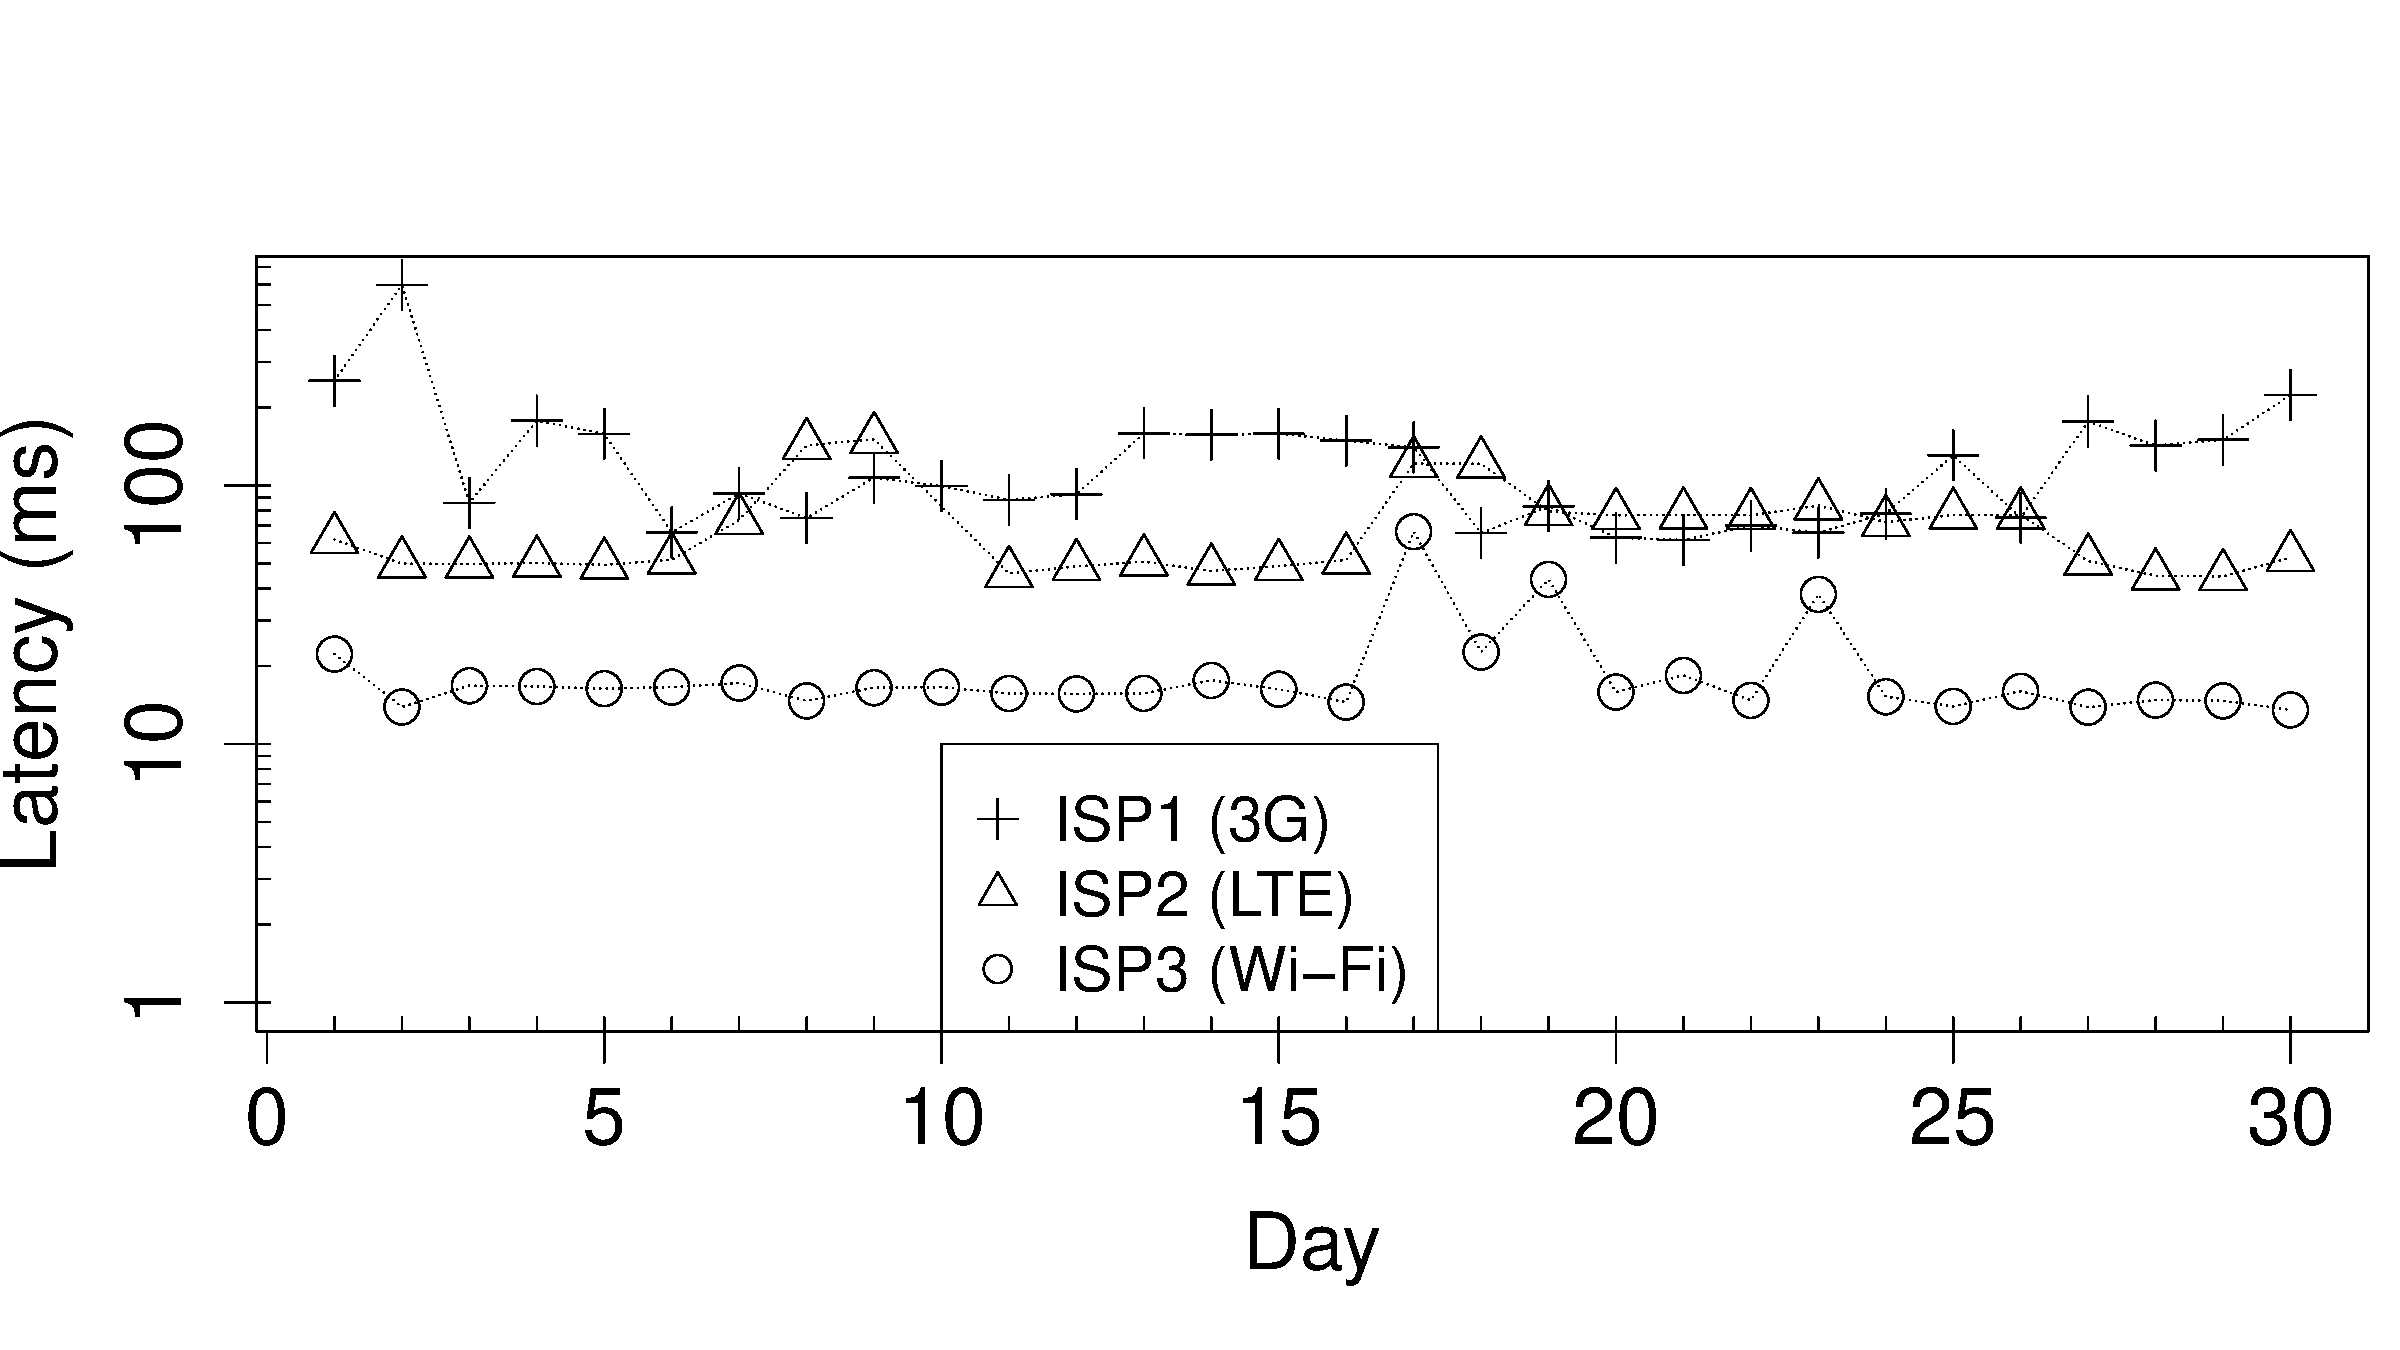
\includegraphics[width=\columnwidth]{plots/compare_isp_latency.pdf}
% \caption{Comparison of ISPs that serve the same user during a 30 day time period. \emph{The LTE service provider has a smaller latency to the 3G provider. The smallest latency is observed by in the home Wi-Fi network.}}
% \label{fig:compare-isp-latency}
% \end{figure}

% \begin{figure}[t]
% 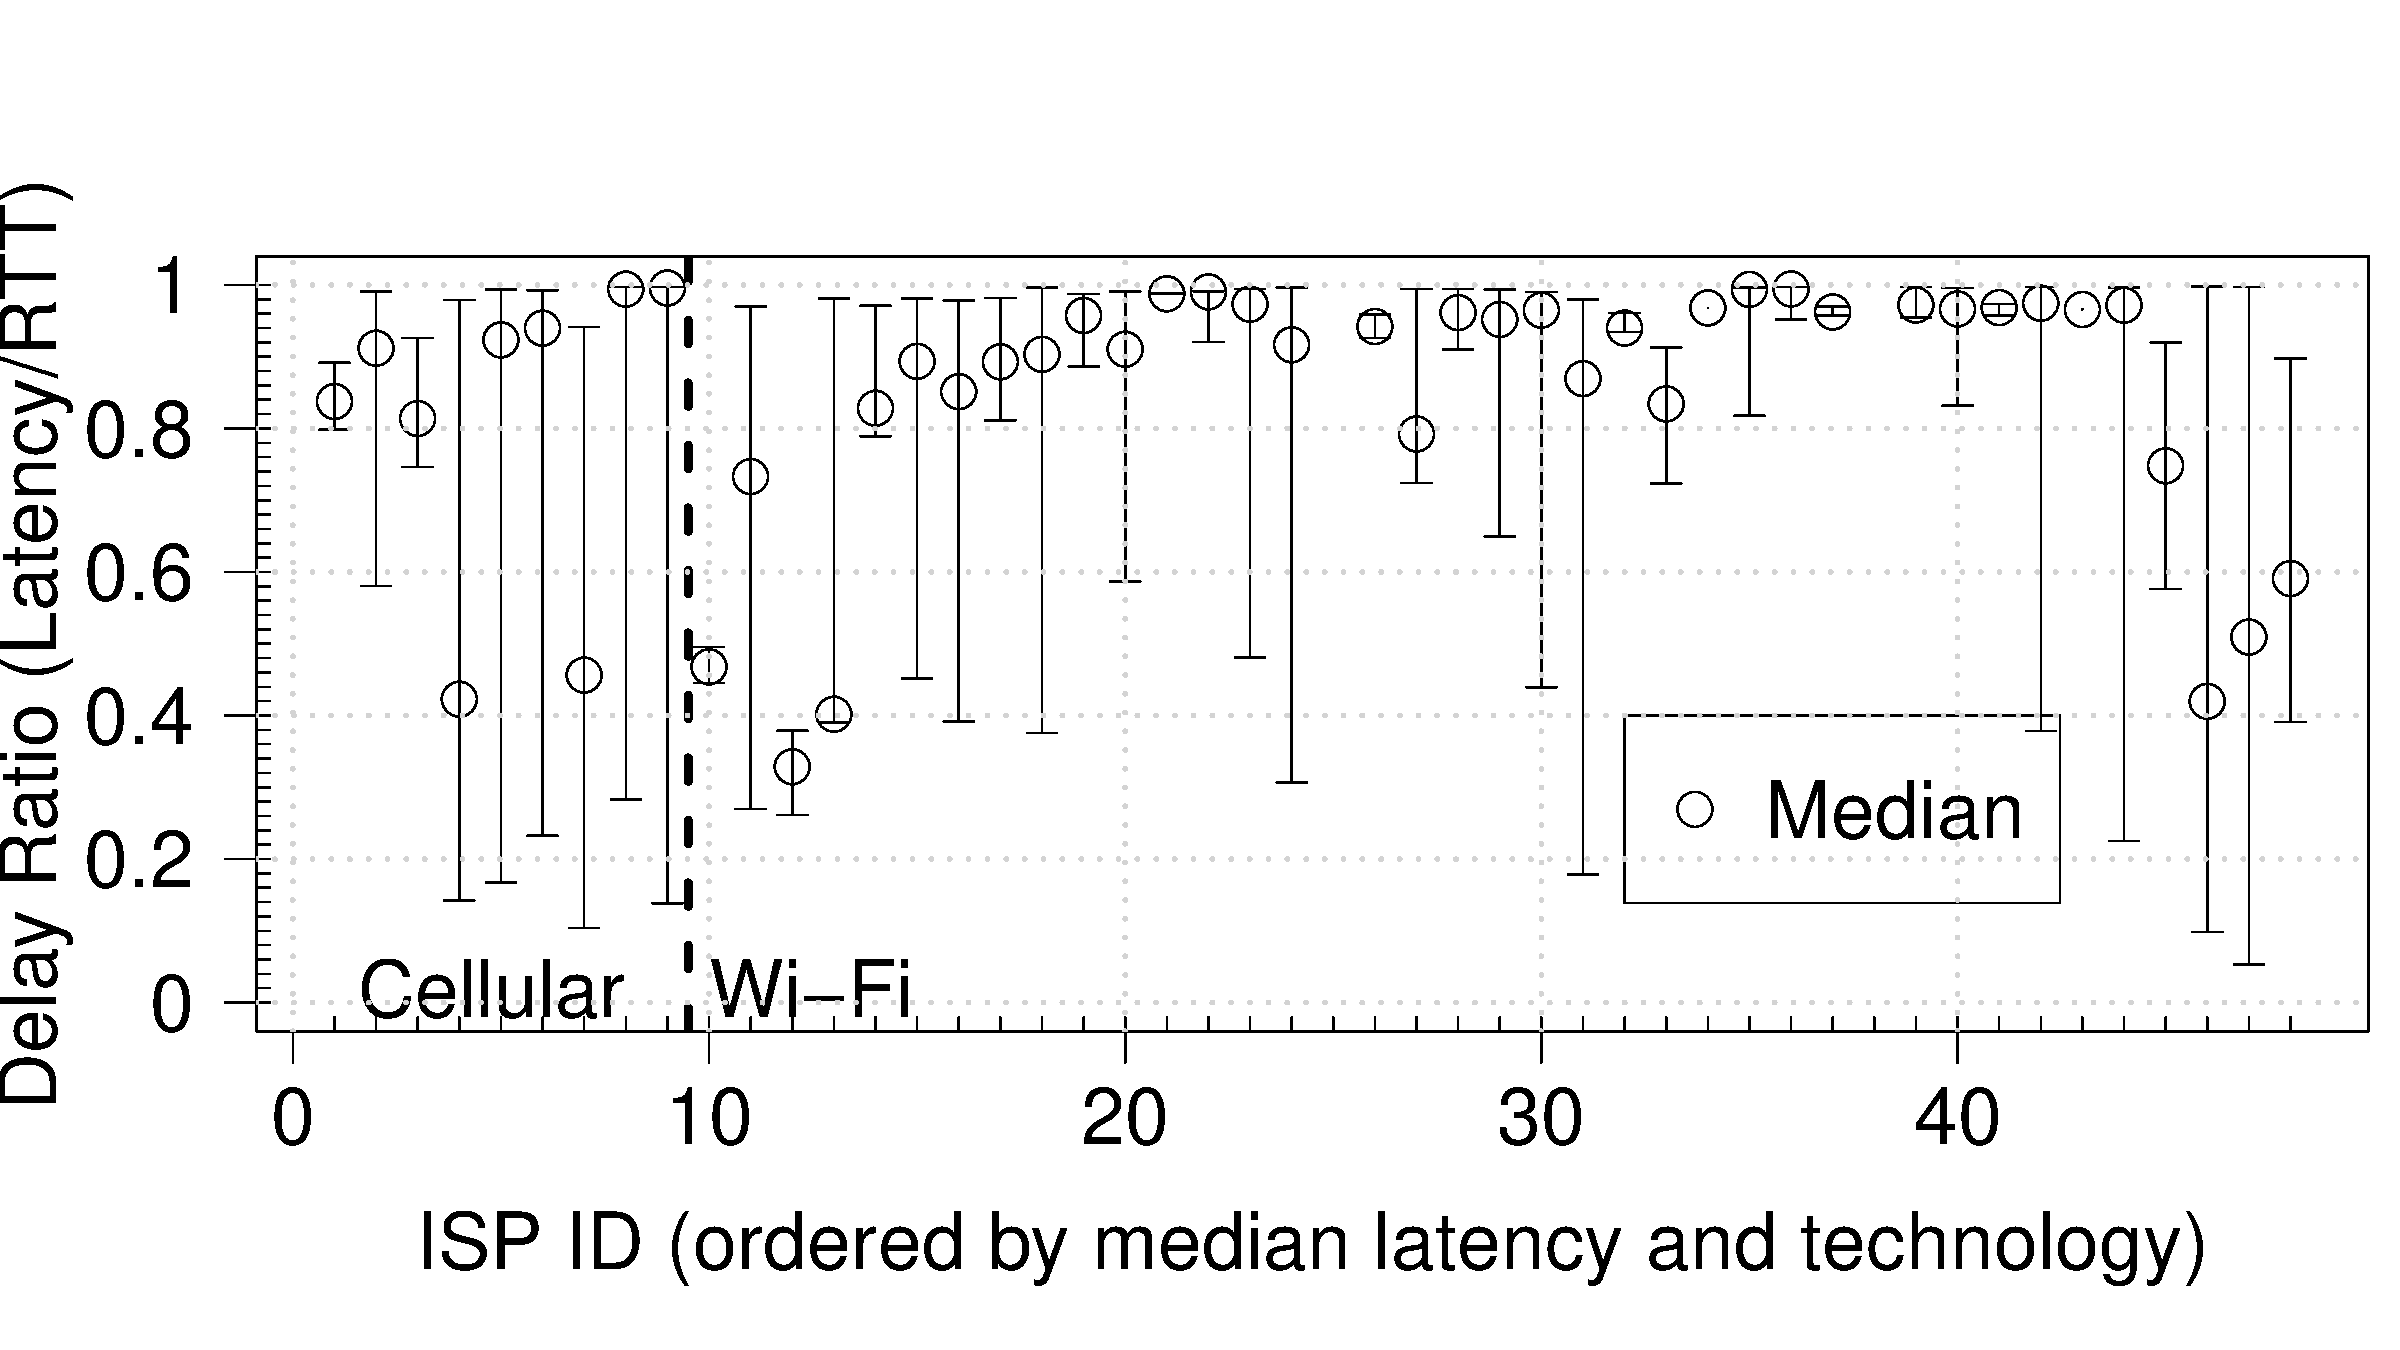
\includegraphics[width=\columnwidth]{plots/delay_ratio_isp_whisker.pdf}
% \caption{Latency as a fraction of the round trip time to contact google services. \emph{In 35 ISPs of the 48 ISPs we observe that the latency of the mobile device to our server accounts for more than 90\% of the end-to-end round trip time. Error bars indicate the 91st and 9th percentile.}}
% \label{fig:compare-delay-ratio}
% \end{figure}

% \begin{figure}[t]
% 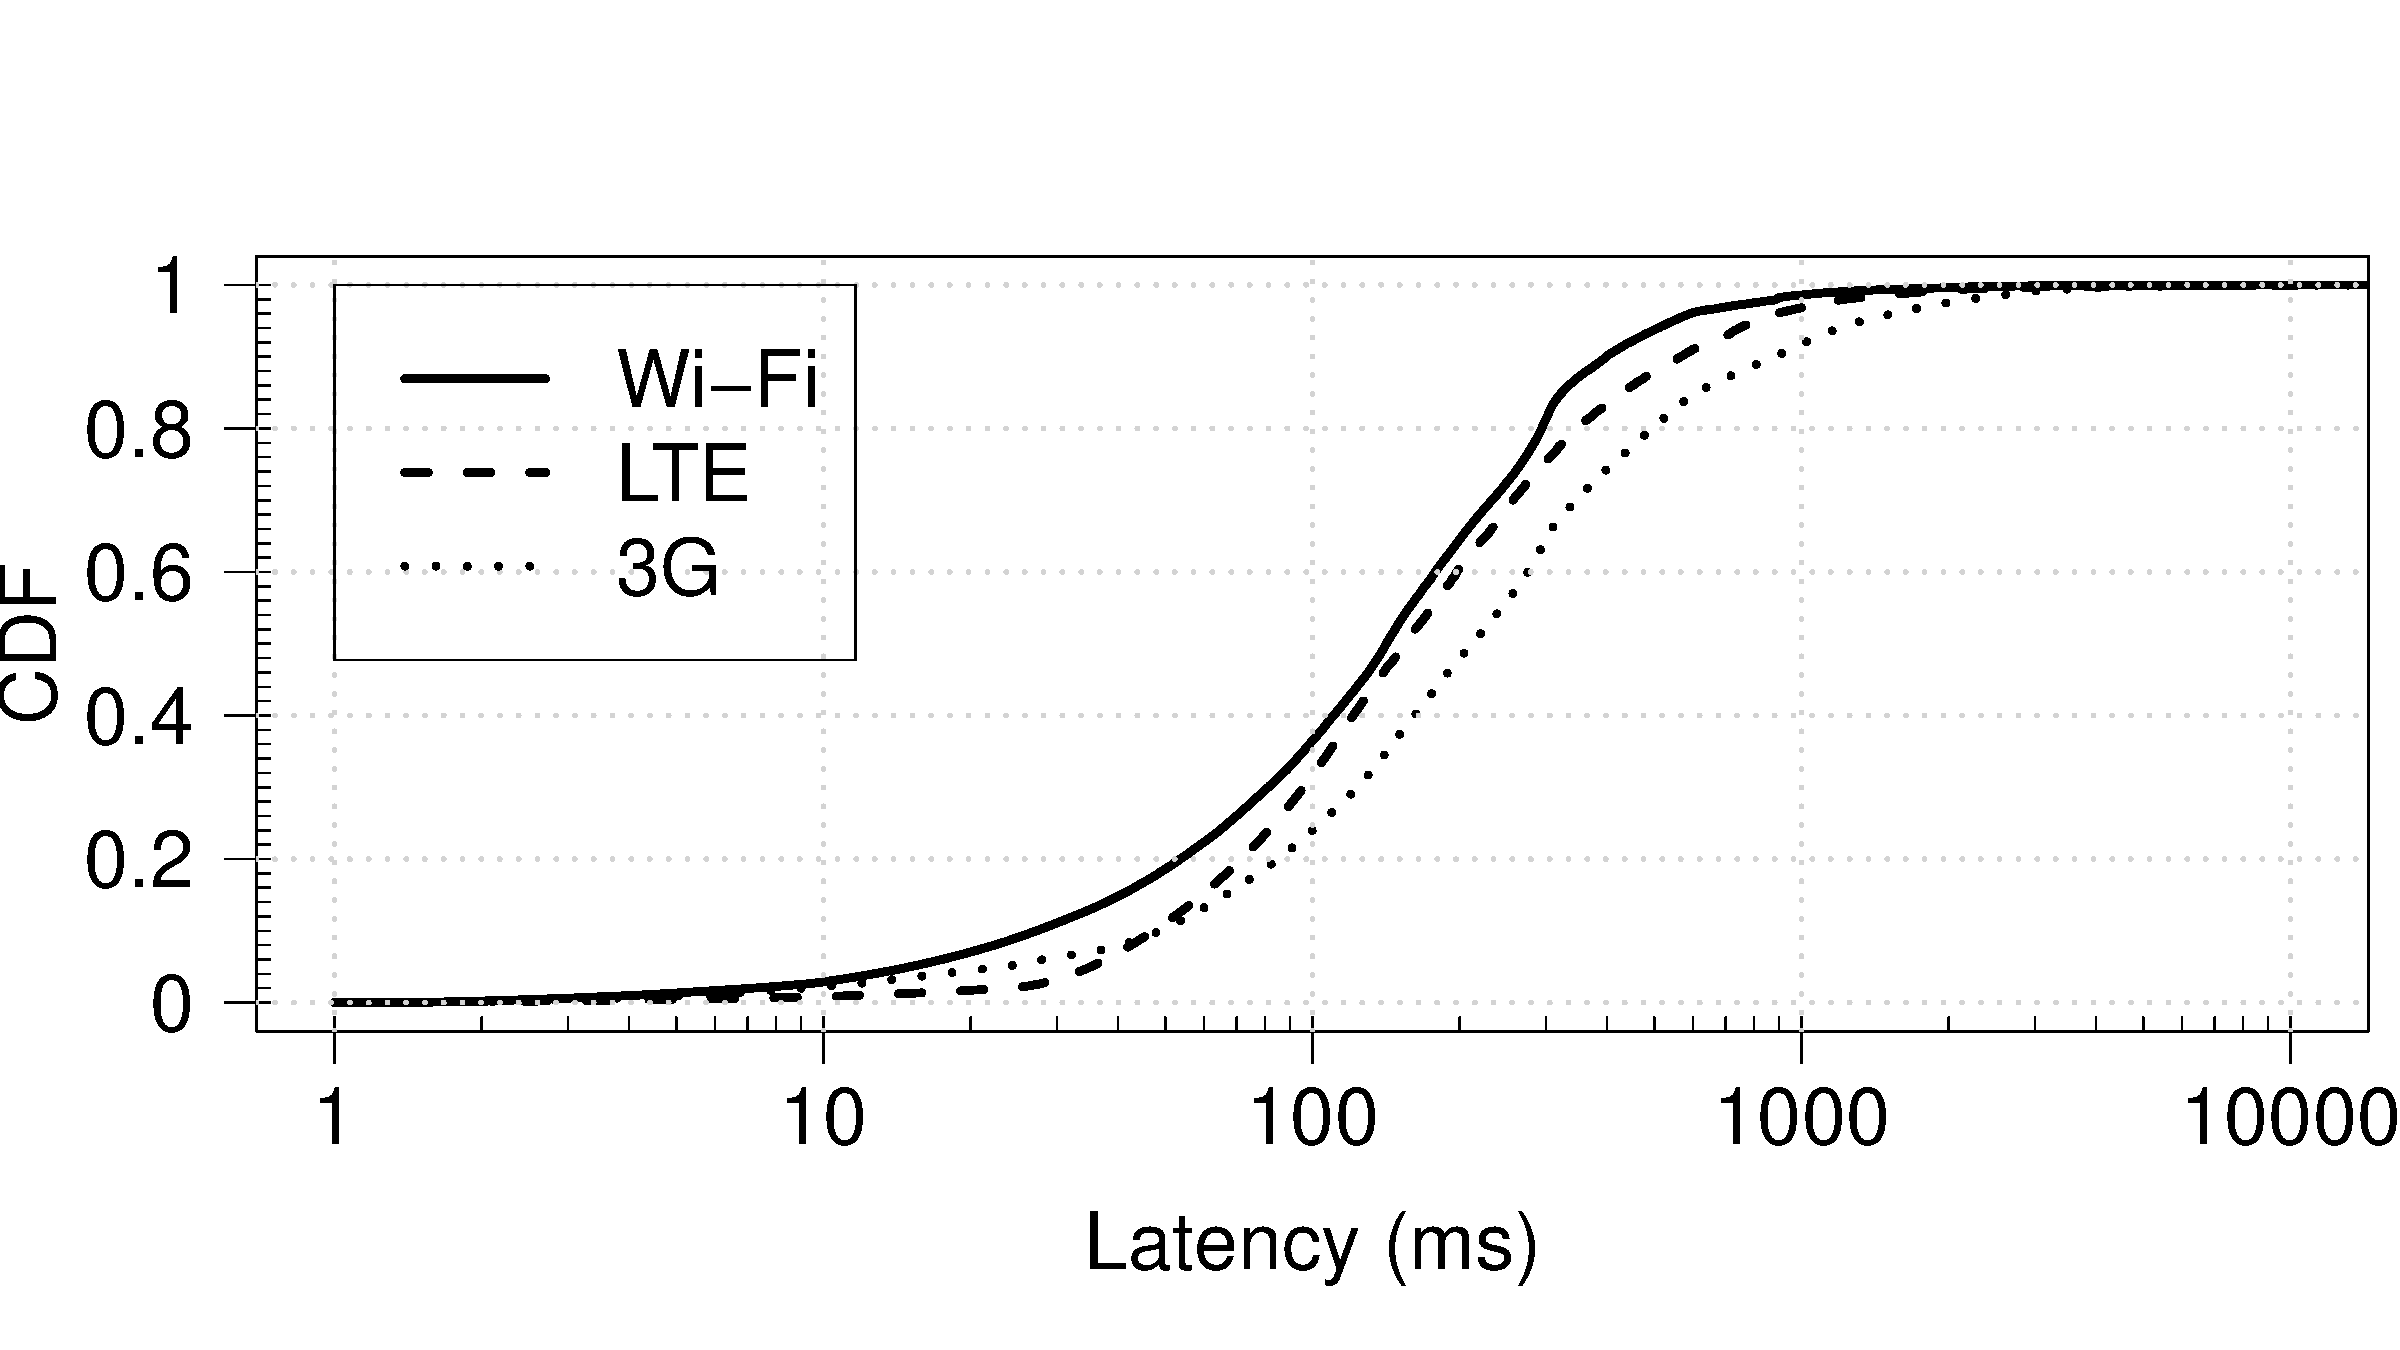
\includegraphics[width=\columnwidth]{plots/distrib_latency_technology.pdf}
% \caption{Distribution of latency over cellular and \wifi ISPs. \emph{The distribution of latency observed when using LTE in the wild is similar to that observed for \wifi}.}
% \label{fig:compare-delay-ratio}
% \end{figure}

% \begin{figure}[t]
% 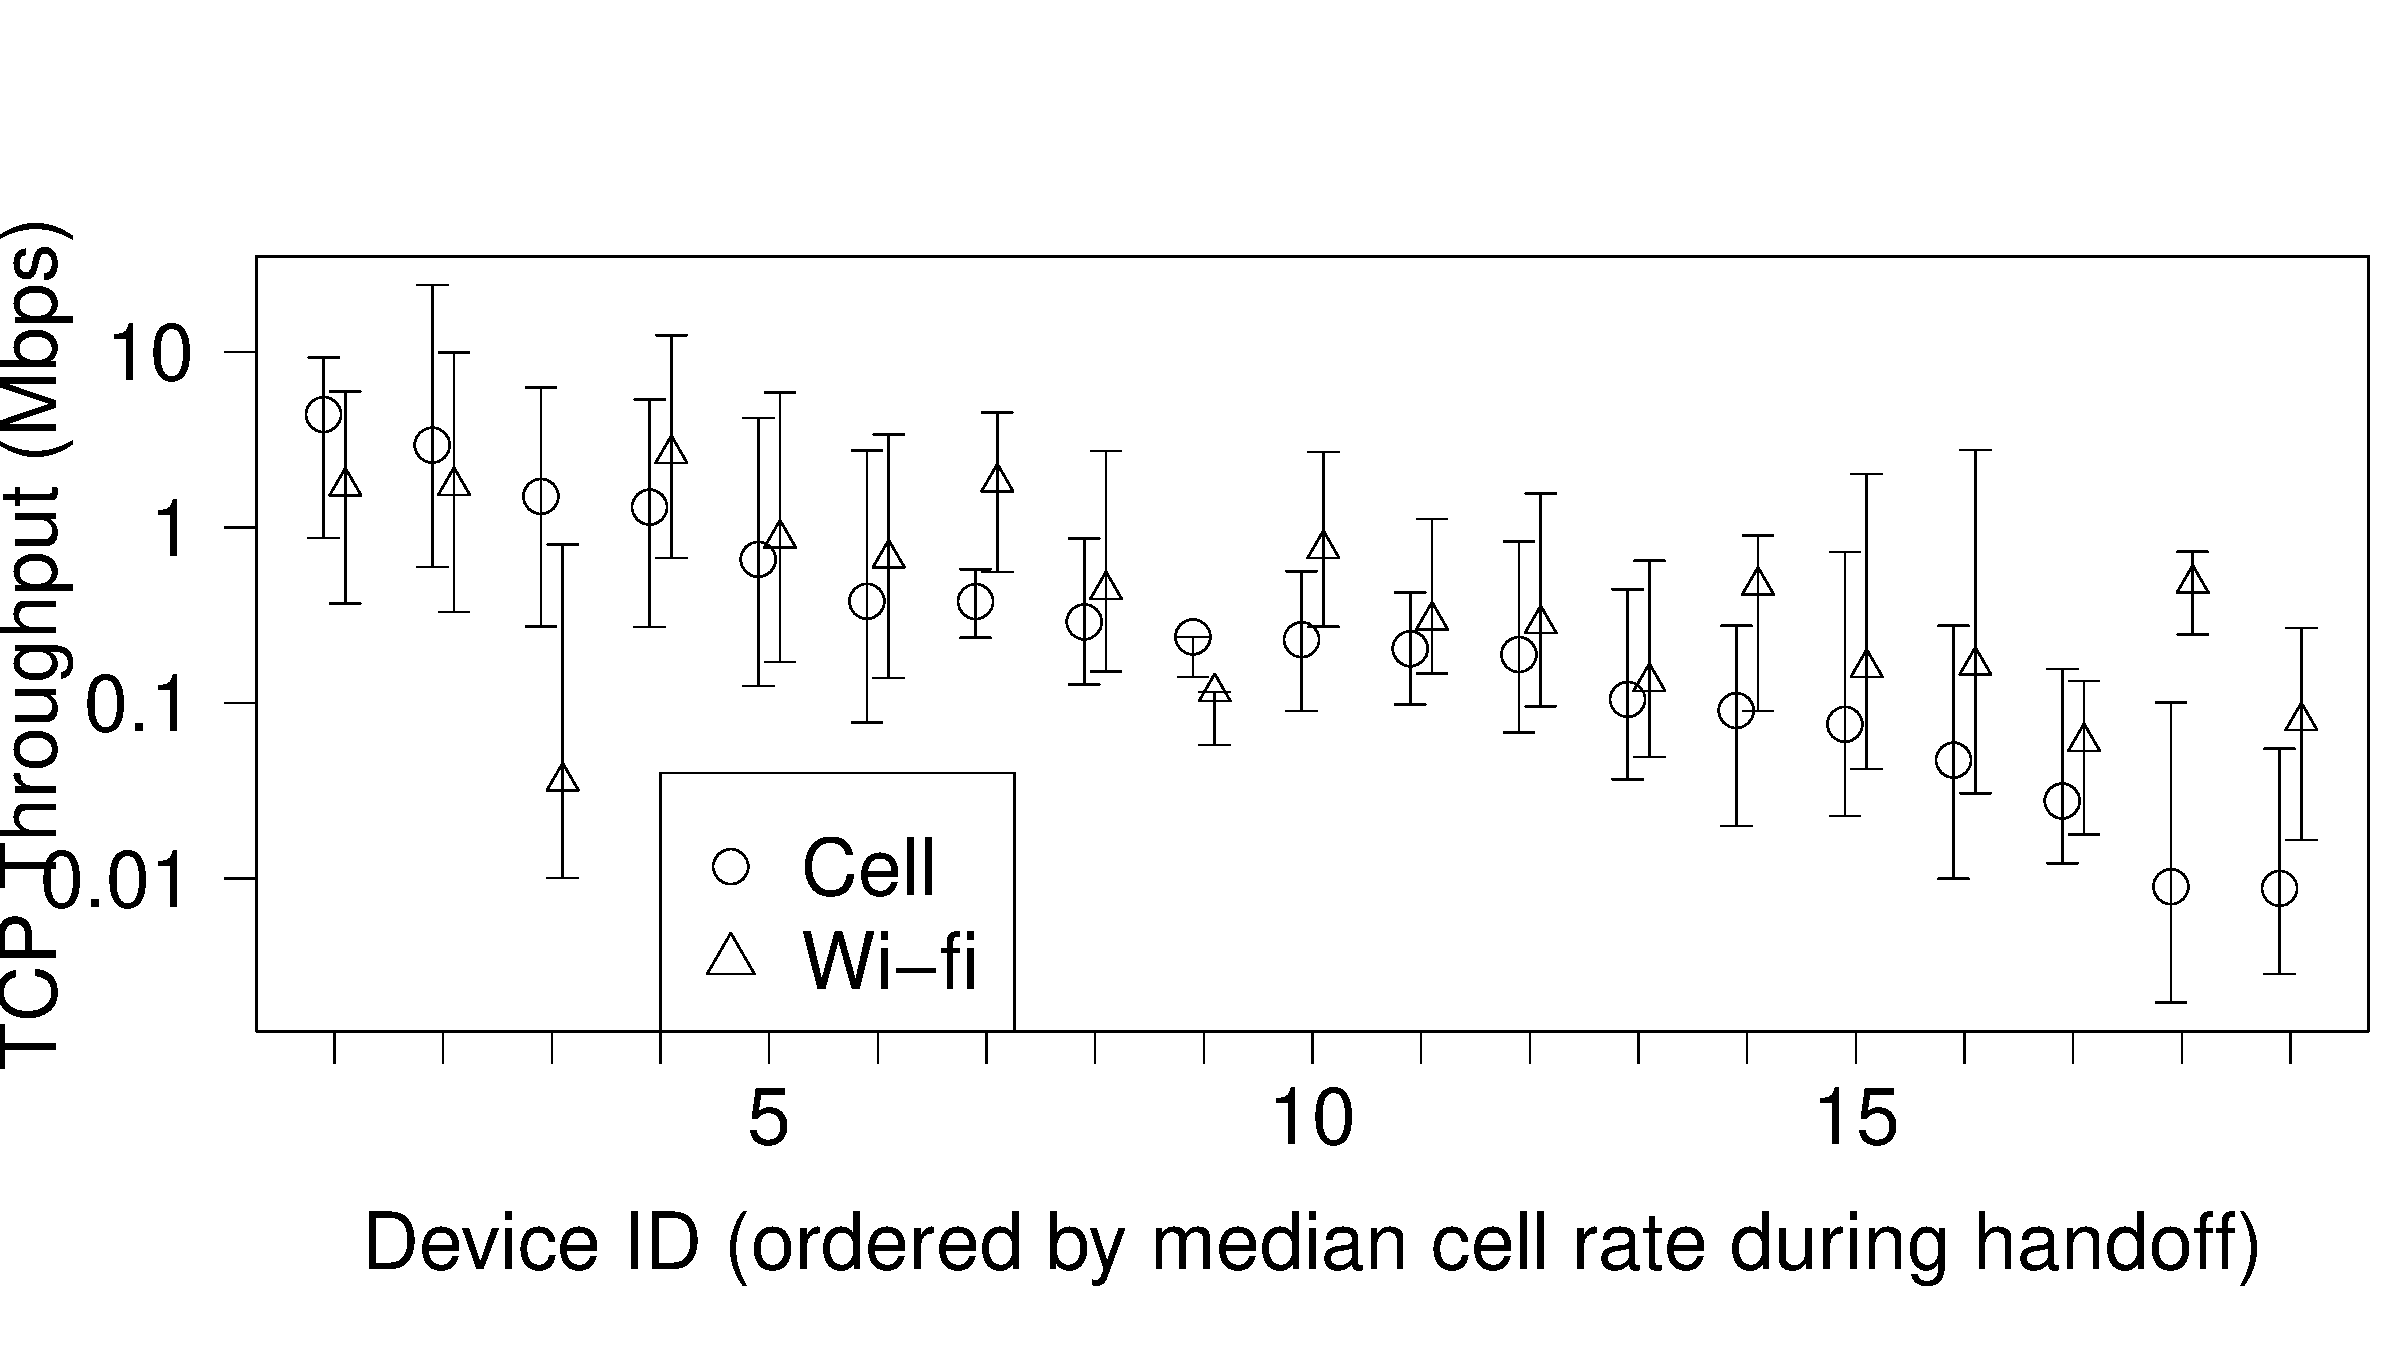
\includegraphics[width=\columnwidth]{plots/handoff_rates.pdf}
% \caption{TCP Throughput observed during the hour of the handoff. \emph{The three users that have LTE connections observed a better TCP throughput over LTE in comparison to \wifi in the hour of the handoff. Error bars indicate the 91st and 9th percentile}.}
% \label{fig:compare-handoff}
% \end{figure}
% \tbd{We performed a traceroute from our server to the egress link and found }

